\documentclass{article}
\usepackage{bm}
\usepackage{amsmath}
\usepackage{graphicx}
\usepackage{mdwlist}
\usepackage[colorlinks=true]{hyperref}
\usepackage{geometry}
\usepackage{kotex}
\geometry{margin=1in}
\geometry{headheight=2in}
\geometry{top=2in}
\usepackage{palatino}
%\renewcommand{\rmdefault}{palatino}
\usepackage{fancyhdr}
\usepackage{indentfirst}
\usepackage{multirow}
\usepackage{tabularx}

\newcommand{\red}[1]{{\color{red} #1}}
\newcommand{\blue}[1]{{\color{blue} #1}}
\newcommand{\orange}[1]{{\color{orange} #1}}
\newcommand{\purple}[1]{{\color{purple} #1}}

%\pagestyle{fancy}
\rhead{}
\lhead{}
\chead{%
  {\vbox{%
      \vspace{2mm}
      \large
      Statistics Lab 033.020\hfill
\\
      Seoul National University
      \\[4mm]
      \textbf{Assignment \#8} \\
      \texttt{2016-19516, Sangjun Son}
    }
  }
}

%%%%%%%%%%%%%%%%%%%%%%%
\usepackage{xcolor}
\usepackage{listings}
\definecolor{vgreen}{RGB}{104,180,104}
\definecolor{vblue}{RGB}{49,49,255}
\definecolor{vorange}{RGB}{255,143,102}

\lstdefinestyle{r-style}
{
    language=R,
    basicstyle=\footnotesize\ttfamily,
    keywordstyle=\color{vblue},
    identifierstyle=\color{black},
    commentstyle=\color{vgreen},
    numbers=left,
    numberstyle=\tiny\color{black},
    numbersep=10pt,
    tabsize=8,
    moredelim=*[s][\colorIndex]{[}{]},
    literate=*{:}{:}1,
    escapeinside=``,
}

\lstdefinestyle{out-style}
{
    basicstyle=\footnotesize\ttfamily,
    numbersep=10pt,
    tabsize=8,
    moredelim=*[s][\colorIndex]{[}{]},
    literate=*{:}{:}1,
    escapeinside=``,
}

\makeatletter
\newcommand*\@lbracket{[}
\newcommand*\@rbracket{]}
\newcommand*\@colon{:}
\newcommand*\colorIndex{%
    \edef\@temp{\the\lst@token}%
    \ifx\@temp\@lbracket \color{black}%
    \else\ifx\@temp\@rbracket \color{black}%
    \else\ifx\@temp\@colon \color{black}%
    \else \color{vorange}%
    \fi\fi\fi
}
\makeatother

\usepackage{trace}
%%%%%%%%%%%%%%%%%%%%%%%

\usepackage{paralist}

\usepackage{todonotes}
\setlength{\marginparwidth}{2.15cm}

\usepackage{tikz}
\usetikzlibrary{positioning,shapes,backgrounds}

\begin{document}

\pagestyle{fancy}

\section*{Example 1}
어느 시장 조사기관은 여러 가지 대중매체가 주는 정보의 양을 비교하기 위해 다음과 
같은 실험을 계획하였다. 40명의 성인을 랜덤하게 추출하여 철저한 면접을 통해 TV, 신문, 
라디오, 잡지 중 어느 매체를 많이 접하는지에 따라 분류하였다. 다음 표는 최근에 일어난 
사건들에 대한 조사 대상자들의 인지도를 측정한 실험에서 얻어진 값들을 나타내고, 값이 
클수록 인지도가 높은 것을 의미한다. 이 자료를 이용하여 사람들의 인지도가 대중매체에 
따라 다르다고 할 수 있는지 유의수준 5\%에서 검정해보자. 

\begin{table}[htb!]
\centering
\begin{tabularx}{0.5\textwidth}{@{\extracolsep{\fill}}cccc}
 \hline
 \multicolumn{4}{c}{조사대상 대중매체} \\ \hline
TV & 신문 & 라디오 & 잡지 \\ \hline
16 & 13 & 18 & 11 \\
19 & 14 & 18 & 15 \\
25 & 15 & 15 & 11 \\
22 & 16 & 14 & 17 \\
21 & 15 & 14 & 17 \\
15 & 13 & 10 & 13 \\
16 & 19 & 18 & 14 \\
22 & 16 & 15 & 16 \\
21 & 20 & 15 & 13 \\
18 & 14 & & 11 \\
& 11 & & \\
\hline
\end{tabularx}
\end{table}

\begin{lstlisting}[style={r-style}]
y = c(16,13,18,11,19,14,18,15,25,15,15,11,22,16,14,17,21,15,14,17,15,13,10,13,16,19,18,14,22,16,
      15,16,21,20,15,13,18,14,11,11)
media = factor(c(rep(1:4,9),1,2,4,2))

df = data.frame(y, media)
fit = lm(y ~ media, data=df)
anova(fit)
\end{lstlisting}
\begin{lstlisting}[style={out-style}]
-------------------------------------------------------------------
Analysis of Variance Table

Response: y
          Df Sum Sq Mean Sq F value    Pr(>F)    
media      3 185.03  61.678  8.2677 0.0002587 ***
Residuals 36 268.56   7.460                      
---
Signif. codes:  0 '***' 0.001 '**' 0.01 '*' 0.05 '.' 0.1 ' ' 1
-------------------------------------------------------------------
\end{lstlisting}
\emph{Explanation: 주어진 자료는 일원배치모형을 적용할 수 있으며 검정하고자 하는 가설은 다음과 같다. 귀무가설 $H_0: \alpha_1=\alpha_2=\alpha_3=\alpha_4=0$과 대립가설 $H_1$: 적어도 한 $\alpha_i$는 0이 아니다. 분산분석을 시행하기 전에 수치변수를 요인(factor)으로 변화하는 과정이 먼저 필요하다. 이를 위해서는 factor() 함수를 사용할 수 있고, 조사대상 대중매체 별로 차이가 있으므로 c()를 이용해 추가되는 데이터의 인덱스를 지정해준다. 분산분석의 시행은 lm() 함수를 사용한다. 분산분석 결과, 검정통계량의 값은 8.2677이고 유의확률은 0.001이하로 매우 작은 것으로 나타났다. 따라서 유의수준 5\%에서 귀무가설을 기각할 수 있다. \textbf{즉, 조사대상 대중매체에 따라 사람들의 인지도에 차이가 있다는 결론을 얻을 수 있다.}} \\

\section*{Example 2}
어느 회사의 마케팅 부서에서는 하나의 상품에 대해 세 가지 다른 디자인의 포장을
적용한 후 이 상품들을 서로 다른 5군데의 상점에서 한 달 동안 판매하였다. 그리고 그 판매
결과는 아래와 같다. 제품의 매출은 판매되는 상점과 제품의 포장 디자인에 따라 다르다고 할
수 있는가? 적절한 가설을 쓰고 유의수준 5\%에서 이를 검정하시오. 

\begin{table}[htb!]
\centering
\begin{tabularx}{0.7\textwidth}{@{\extracolsep{\fill}}c|ccccc}
& 상점 1 & 상점 2 & 상점 3 & 상점 4 & 상점 5 \\ \hline
상자 1 & 210 & 230 & 190 & 180 & 190 \\
상자 2 & 195 & 170 & 200 & 190 & 193 \\
상자 3 & 295 & 275 & 290 & 275 & 265 \\
\end{tabularx}
\end{table}
\begin{lstlisting}[style={r-style}]
y = c(210,230,190,180,190,195,170,200,190,193,295,275,290,275,265)
A = rep(c("S1","S2","S3","S4","S5"), 3)
B = rep(c("B1","B2","B3"), rep(5,3))

df = data.frame(A, B, y)
fit = lm(y ~ A+B, data=df)
anova(fit)
\end{lstlisting}
\begin{lstlisting}[style={out-style}]
-------------------------------------------------------------------                 
Analysis of Variance Table

Response: y
          Df  Sum Sq Mean Sq F value    Pr(>F)    
A          4   711.1   177.8  0.7033    0.6114    
B          2 24467.2 12233.6 48.3988 3.396e-05 ***
Residuals  8  2022.1   252.8 
---
Signif. codes:  0 '***' 0.001 '**' 0.01 '*' 0.05 '.' 0.1 ' ' 1
-------------------------------------------------------------------
\end{lstlisting}
\emph{Explanation: 주어진 자료는 반복이 없는 이원배치법 모형이 적용 가능하며 상점에 따른 효과를 $\alpha_i$
라고 하고 제품의 포장 디자인에 따른 효과를 $\beta_i$ 라고 하면 검정하고자 하는 가설은 다음과 같다. (인자 A에 대한) 귀무가설 $H_0: \alpha_1=\alpha_2=\alpha_3=\alpha_4=\alpha_5=0$과 대립가설 $H_1$: 적어도 한 $\alpha_i$는 0이 아니다. (인자 B에 관한) 귀무가설 $H_0: \beta_1=\beta_2=\beta_3=0$과 대립가설 $H_1$: 적어도 한 $\beta_i$는 0이 아니다. 이번에는 예제 1번과 사뭇 다른 방법으로 factor를 지정해 준다. 제품의 매출의 관측값 y를 2개의 요인에 나누어 저장하기 위해 처음부터 문자열의 형태로 rep() 반복을 써서 저장을 한다. 이렇게 하면 요인 A와 요인 B의 인자 수준을 숫자로 입력했으므로 수치변수를 요인으로 변환하는 과정을 거칠 필요가 없어질 것이고 Dataframe을 생성했을 때 가독성 또한 
높아지는 장점이 있다. 분산분석은 lm() 함수를 사용해서 시행할 수 있고, 두 개의 요인은 '+'기호로 연결한다. 분산분석표 확인 결과, 상점 (A)의 효과에 대한 유의 확률은 0.6114로 유의수준 0.05보다 높고 포장 디자인 (B)의
효과에 대한 유의 확률은 3.396e-05로 유의수준보다 낮다. \textbf{따라서 포장 디자인에 따른 제품 매출은 유의한 차이를 낸다고 볼 수 있으나 상점에 따라 제품 매출이 달라진다고 할 수 없다.} } \\

\section*{Example 3}
남녀의 성별과 고단백질로 구성된 아침 식사의 섭취 여부가 성인의 신체적 활동
능력에 영향을 미치는지를 알아보기 위하여 랜덤하게 선택된 남녀 10명에 대해 각각 5명씩
고단백질 아침식사와 저단백질 아침식사를 섭취하게 한 후, 신체적 능력을 테스트를 통해
측정하였다. 측정된 점수가 높을수록 신체 활동 능력이 더 우수하다는 것을 의미한다. 실험
결과가 아래와 같을 때, 주어진 자료에 대해 이원배치법을 적용한 후 그 결과를 해석하여라.

\begin{table}[htb!]
\centering
\begin{tabularx}{0.4\textwidth}{@{\extracolsep{\fill}}c|cc} \hline
& 고단백질 식사 & 저단백질 식사 \\ \hline
남성 & 10 7 9 6 8 & 5 4 7 4 5 \\ \hline
여성 & 5 4 6 3 2 & 3 4 5 1 2  \\ \hline
\end{tabularx}
\end{table}

\begin{lstlisting}[style={r-style}]
y = c(10,7,9,6,8,5,4,7,4,5,5,4,6,3,2,3,4,5,1,2)
A = rep(c("`고`","`저`","`고`","`저`"), rep(5,4))
B = rep(c("`남`","`여`"), rep(10,2))

df = data.frame(A, B, y)
fit = lm(y ~ A*B, data=df)
anova(fit)
\end{lstlisting}
\begin{lstlisting}[style={out-style}]
-------------------------------------------------------------------         
Analysis of Variance Table

Response: y
          Df Sum Sq Mean Sq F value    Pr(>F)    
A          1     20   20.00  8.8889 0.0088144 ** 
B          1     45   45.00 20.0000 0.0003851 ***
A:B        1      5    5.00  2.2222 0.1554875    
Residuals 16     36    2.25
---
Signif. codes:  0 '***' 0.001 '**' 0.01 '*' 0.05 '.' 0.1 ' ' 1
-------------------------------------------------------------------
\end{lstlisting}
\emph{Explanation: (반복이 있는 이원배치법의 모형) 고단백질로 구성된 아침 식사의 섭취 여부를 $\alpha_i$, 남녀의 성별에 따른 효과를 $\beta_i$, 아침 식사의 섭취와 성별의 상호작용을 $\gamma_{ij}$ 라고 하면 검정하고자 하는 가설은 다음과 같다.
(요인 A에 대한) 귀무가설 $H_0: \alpha_1=\alpha_2=0$과 대립가설 $H_1$: 적어도 한 $\alpha_i$는 0이 아니다. (요인 B에 대한) 귀무가설 $H_0: \beta_1=\beta_2=0$과 대립가설 $H_1$: 적어도 한 $\beta_i$는 0이 아니다. (교호작용에 대한) 귀무가설 $H_0: \gamma_{11}=\gamma_{12}=\gamma_{21}=\gamma_{22}=0$과 대립가설 $H_1$: 적어도 한 $\gamma_{ij}$는 0이 아니다. 상호작용을 포함하는 이원배치 분산분석은 두 개의 요인을 곱(*)으로 표현하여 실행할 수 있다. 분산분석 결과, 유의수준 5\%에서 \textbf{고단백질로 구성된 아침 식사의 섭취 여부 (A)와 남녀의 성별 (B)에 따른 상호작용은 존재하지 않는 것}으로 나타났다 (F=2.2222, p-value$>$0.05). 
하지만 \textbf{고단백질로 구성된 아침 식사의 섭취 여부 (A)와 남녀의 성별 (B) 각각의 요인에 따라서 신체 활동 능력의 차이가 유의하다}고 할 수 있다. (p-value$<$0.05). } \\

\section*{Example 4}
서로 다른 네 종류의 비료의 효과를 비교하기 위해 세 지역에 같은 작물을 심고 수확량을
비교하였다. 수확량은 다음과 같다. 

\begin{table}[htb!]
\centering
\begin{tabularx}{0.5\textwidth}{@{\extracolsep{\fill}}|c|ccc|} \hline
변수명 & region1 & region2 & region3 \\ \hline
fertilizer1 & 12.1 & 12.8 & 13.9  \\ \hline
fertilizer2 & 13.6 & 18.4 & 17.5  \\ \hline
fertilizer3 & 14.2 & 17.2 & 19.2  \\ \hline
fertilizer4 & 21.7 & 21.4 & 17.5  \\ \hline

\end{tabularx}
\end{table}

비료에 따라 수확량이 달라진다고 할 수 있는가? 적절한 가설을 쓰고 유의수준 5\%에서 이를 검정하시오.

\begin{lstlisting}[style={r-style}]
y = c(12.1,12.8,13.9,13.6,18.4,17.5,14.2,17.2,19.2,21.7,21.4,17.5)
A = rep(c("R1","R2","R3"), 4)
B = rep(c("F1","F2","F3","F4"), rep(3,4))

df = data.frame(A, B, y)
fit = lm(y ~ A+B, data=df)
anova(fit)
\end{lstlisting}
\begin{lstlisting}[style={out-style}]
-------------------------------------------------------------------    
Analysis of Variance Table

Response: y
          Df Sum Sq Mean Sq F value  Pr(>F)  
A          2  9.365  4.6825  0.9705 0.43134  
B          3 79.449 26.4831  5.4890 0.03724 *
Residuals  6 28.948  4.8247 
---
Signif. codes:  0 '***' 0.001 '**' 0.01 '*' 0.05 '.' 0.1 ' ' 1
-------------------------------------------------------------------
\end{lstlisting}
\emph{Explanation: 주어진 자료는 반복이 없는 이원배치법 모형이 적용 가능하나 결론을 내리기 위해서는 두 요인 중 한 요인 (비료)이 수확량에 따른 효과가져 오는지에 관한 가설 검정을 하면 된다. 지역에 따른 효과를 $\alpha_i$
라고 하고 네 가지 비료에 따른 효과를 $\beta_i$ 라고 하면 검정하고자 하는 가설은 다음과 같다. (인자 A에 대한) 귀무가설 $H_0: \alpha_1=\alpha_2=\alpha_3=0$과 대립가설 $H_1$: 적어도 한 $\alpha_i$는 0이 아니다. (인자 B에 관한) 귀무가설 $H_0: \beta_1=\beta_2=\beta_3=\beta_4=0$과 대립가설 $H_1$: 적어도 한 $\beta_i$는 0이 아니다. 
이전 예제와 마찬가지 방법으로 factor를 지정해주고 분산분석 lm()을 시행한다. 이 때, 두 개의 요인은 '+'기호로 연결한다. 분산분석 결과, 지역 (A)의 효과에 대한 유의 확률은 0.43134로 유의수준 0.05보다 높고 비료 (B)의
효과에 대한 유의 확률은 0.03724로 유의수준보다 낮다. \textbf{따라서 비료에 따른 수확량은 유의한 차이를 낸다고 볼 수 있다.}} \\

\section*{Example 5}
\texttt{mlb\_players\_18}는 2018 시즌 미국 메이저리그에서 100타석 이상의 기록이 있는 타자 429명의
통계를 정리한 자료이다. \texttt{mlb\_players\_18} 자료는 다음의 변수들로 이루어져 있다.
\begin{itemize}
  \setlength\itemsep{-0.4em}
    \item \texttt{name}: 선수 이름
    \item \texttt{team}: 소속 팀
    \item \texttt{position}: 선수의 수비 위치 (C, 1B, 2B, 3B, LF, CF, RF, SS)
    \item \texttt{AB}: 타석 수
    \item \texttt{H}: 총 안타 수 (아래 \texttt{doubles}, \texttt{triples}, \texttt{HR} 개수를 모두 포괄한 수치)
    \item \texttt{doubles}: 총 2루타 수
    \item \texttt{triples}: 총 3루타 수
    \item \texttt{HR}: 총 홈런 수
    \item \texttt{AVG}: 타율
    \item \texttt{OBP}: 출루율
\end{itemize}
이 문제에서는 선수의 수비 위치에 따라 타율이 달라지는지 검정하고자 한다. \\

\textbf{(1)} 선수의 수비 위치에 따른 타율을 상자그림으로 표현해보자. 수비 위치에 따라 타율이 다르다고 예상할 수 있는가?

\begin{lstlisting}[style={r-style}]
mlb_players_18 = read.csv("mlb_players_18.csv", header=T)
boxplot(AVG ~ position, data=mlb_players_18, main="`선수의 수비 위치에 따른 타율`")
\end{lstlisting}
\begin{figure}[htb!]
    \centering
    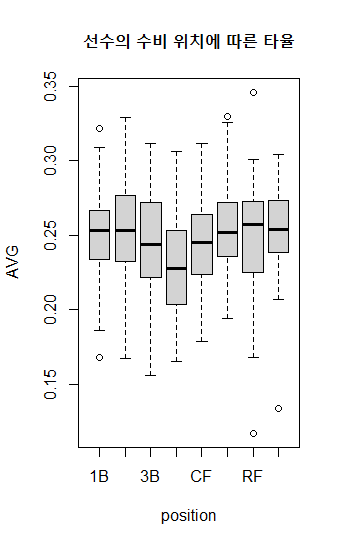
\includegraphics[width=0.4\textwidth]{fig/ex5-1.png}
\end{figure}
\emph{Explanation: 먼저 "mlb\_players\_18.csv"로부터 데이터를 읽어온다. 이전에 배웠던 상자그림을 그릴 때 사용하는 함수 boxplot()을 활용하여 선수의 수비위치 position에 따른 타율 AVG를 데이터셋 mlb\_players\_18에 대하여 기술한 결과는 위 도식과 같다. 수비 위치에 따라 타율의 평균값 및 분포가 각기 다르므로 \textbf{선수의 수비 위치에 따라 타율이 달라지는 검정 결과}를 예상할 수 있다.} \\

\textbf{(2)} 수비 위치가 같은 선수들의 타율이 정규분포를 따르는지 분위수대조도를 이용해 설명하시오.

\begin{lstlisting}[style={r-style}]
par(mfrow=c(3,3))
for (pos in c("C","1B","2B","3B","LF","CF","RF","SS")) {
  data = mlb_players_18[mlb_players_18$position==pos,]
  qqnorm(data$AVG, main=paste("Q-Q plot for", pos))
  qqline(data$AVG, col=2, lwd=2)
}
dev.off()
\end{lstlisting}
\begin{figure}[htb!]
    \centering
    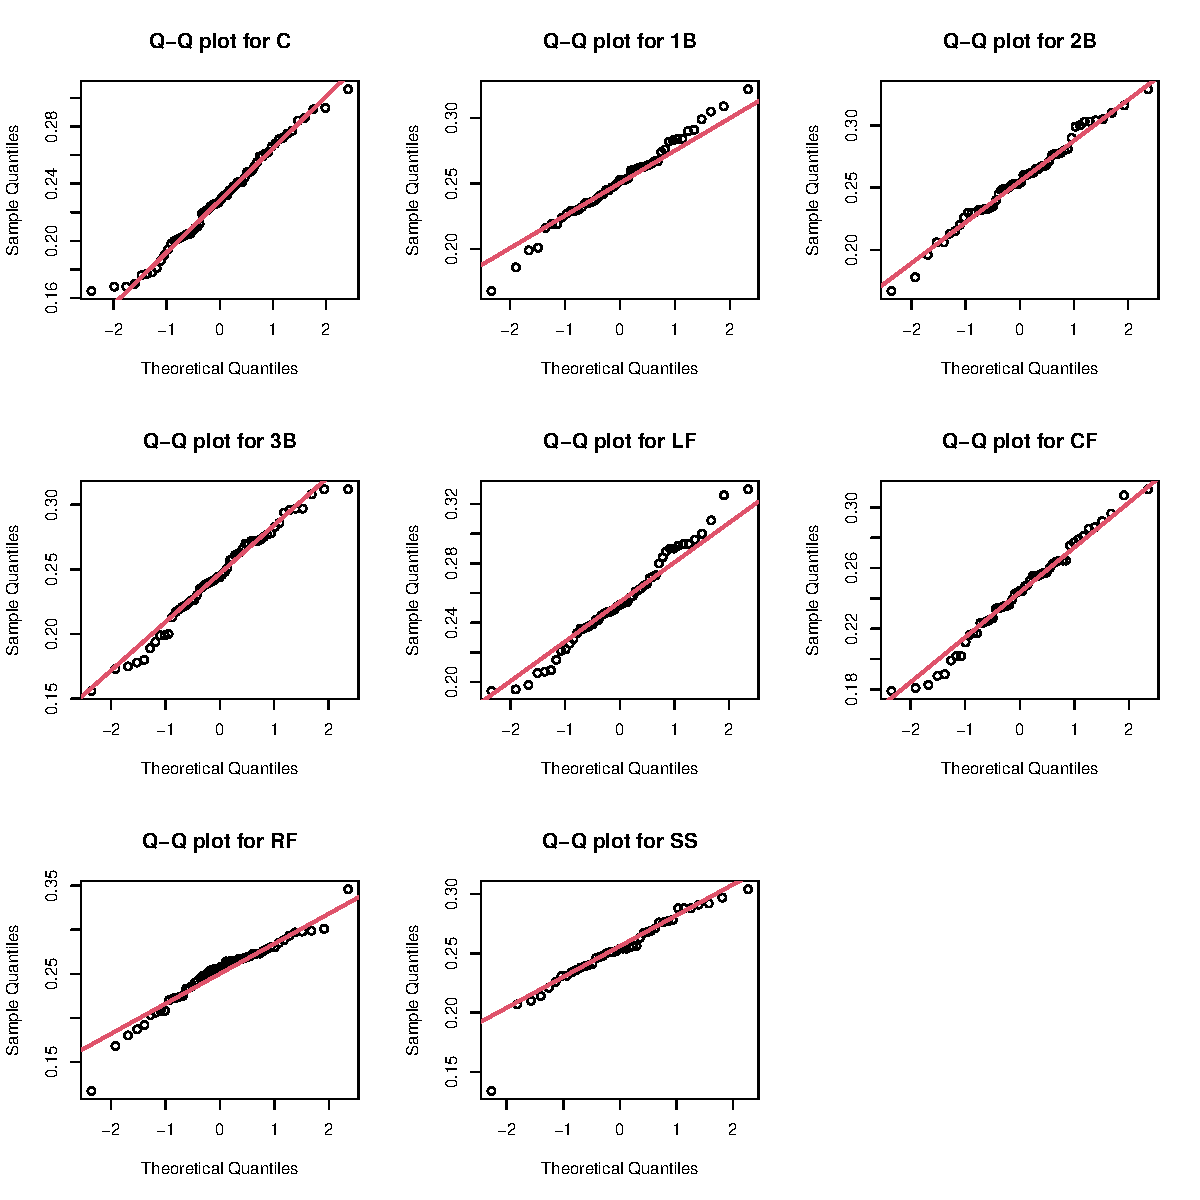
\includegraphics[width=\textwidth]{fig/ex5-2.pdf}
\end{figure}
\newpage
\emph{Explanation: 선수의 수비 위치의 항목 갯수 (C, 1B, 2B, 3B, LF, CF, RF, SS: 총 8개) 만큼 정규분포 분위수대조도를 그려야 하므로 3*3 차트 영역을 생성해준다. 각각의 포지션에 맞는 선수들을 filtering 하여 data에 저장한다. 이전 장에서 배웠던 QQ plot을 하기 위한 함수 qqnorm()과 qqline()을 이용하여 data에 저장된 선수들의 타율 AVG 값에 대한 정규분포 분위수 대조를 진행한다. 대체적으로 QQ line에 잘 분포되어 있는 것으로 보아 \textbf{모집단이 정규분포를 따른다고 가정할 수 있다.}} \\

\newpage
\textbf{(3)} 적절한 가설을 쓰고 유의수준 5\%에서 이를 검정하시오

\begin{lstlisting}[style={r-style}]
fit = lm(AVG ~ position, data=mlb_players_18)
anova(fit)
\end{lstlisting}
\begin{lstlisting}[style={out-style}]
-------------------------------------------------------------------    
Analysis of Variance Table

Response: AVG
           Df  Sum Sq   Mean Sq F value    Pr(>F)    
position    7 0.03207 0.0045819  3.9125 0.0003789 ***
Residuals 421 0.49303 0.0011711  
---
Signif. codes:  0 '***' 0.001 '**' 0.01 '*' 0.05 '.' 0.1 ' ' 1
-------------------------------------------------------------------
\end{lstlisting}
\emph{Explanation: 주어진 자료는 일원배치모형을 적용할 수 있으며 검정하고자 하는 가설은 다음과 같다. 포지션에 따른 효과를 $\alpha_i$라고 할 때 귀무가설 $H_0: \alpha_i=0$과 대립가설 $H_1$: 적어도 한 $\alpha_i$는 0이 아니다. 분산분석의 시행은 lm() 함수를 사용한다. 분산분석 결과, 검정통계량의 값은 3.9125이고 유의확률은 0.001이하로 매우 작은 것으로 나타났다. 따라서 유의수준 5\%에서 position에 따른 타율 AVG에 대한 효과가 존재하지 않는다는 귀무가설을 기각할 수 있다. \textbf{즉, 수비 위치에 따른 타율의 차이가 있다는 결론을 얻을 수 있다.}} \\

\section*{Example 6}
\texttt{MASS::Boston}은 Boston의 506개 지역의 주택 가격에 대한 데이터이다. \texttt{Boston} 데이터는 다음의 변수를 포함하고 있다. 

\begin{itemize}
  \setlength\itemsep{-0.4em}
    \item \texttt{medv}: 주택 가격의 중앙값 (단위: \$1000)
    \item \texttt{age}: 1940년 이전에 지어진 주택의 비율 (단위: \%)
    \item \texttt{chas} : Chales River에 대한 더미 변수 (접해 있을 때 1, 그 외에 0)
\end{itemize}
이 문제에서는 chas와 age가 가격 medv에 영향을 미치는지 확인하고자 한다.\\

\textbf{(1)} \texttt{age} 변수를 세 그룹으로 나누어 \texttt{Boston\$age\_group}이라는 변수로 저장하자. 비율이 50\%
이하이면 low, 50\% 초과 90\% 이하이면 medium, 90\% 초과이면 high로 저장하시오.

\begin{lstlisting}[style={r-style}]
Boston = MASS::Boston
Boston$age_group = ""
Boston[Boston$age<=50,]$age_group = "low"
Boston[Boston$age>50 & Boston$age<=90,]$age_group = "medium"
Boston[Boston$age>90,]$age_group = "high"
Boston$age_group
\end{lstlisting}
\begin{lstlisting}[style={out-style}]
  [1] "medium" "medium" "medium" "low"    "medium" "medium" "medium"
  [8] "high"   "high"   "medium" "high"   "medium" "low"    "medium"
 [15] "medium" "medium" "low"    "medium" "low"    "medium" "high"  
 [22] "medium" "high"   "high"   "high"   "medium" "high"   "medium"
 [29] "high"   "medium" "high"   "high"   "medium" "high"   "high"  
 [36] "medium" "medium" "low"    "low"    "low"    "low"    "low"   
 [43] "low"    "low"    "low"    "low"    "low"    "medium" "high"  
 [50] "medium" "low"    "medium" "low"    "low"    "low"    "low"   
 [57] "low"    "low"    "low"    "low"    "medium" "high"   "medium"
 [64] "low"    "medium" "low"    "low"    "low"    "low"    "low"   
 [71] "low"    "low"    "low"    "low"    "low"    "low"    "medium"
 [78] "low"    "medium" "low"    "low"    "medium" "low"    "low"   
 [85] "low"    "medium" "low"    "medium" "medium" "medium" "medium"
 [92] "medium" "medium" "low"    "medium" "medium" "medium" "medium"
 [99] "low"    "medium" "medium" "medium" "medium" "medium" "medium"
[106] "high"   "high"   "medium" "high"   "high"   "medium" "medium"
[113] "high"   "high"   "medium" "medium" "medium" "medium" "medium"
[120] "medium" "medium" "medium" "high"   "high"   "high"   "medium"
[127] "high"   "high"   "high"   "high"   "high"   "high"   "high"  
[134] "high"   "high"   "high"   "high"   "high"   "high"   "high"  
[141] "high"   "high"   "high"   "high"   "high"   "high"   "high"  
[148] "high"   "high"   "high"   "high"   "high"   "medium" "high"  
[155] "high"   "medium" "high"   "high"   "high"   "high"   "high"  
[162] "high"   "high"   "high"   "high"   "high"   "high"   "medium"
[169] "high"   "high"   "high"   "high"   "medium" "medium" "medium"
[176] "low"    "low"    "medium" "medium" "medium" "medium" "medium"
[183] "high"   "high"   "medium" "medium" "medium" "low"    "low"   
[190] "low"    "low"    "low"    "low"    "low"    "low"    "low"   
[197] "low"    "low"    "low"    "low"    "low"    "low"    "low"   
[204] "low"    "low"    "low"    "medium" "medium" "medium" "high"  
[211] "high"   "medium" "medium" "low"    "low"    "low"    "medium"
[218] "medium" "high"   "high"   "medium" "high"   "medium" "medium"
[225] "medium" "medium" "medium" "medium" "low"    "low"    "medium"
[232] "medium" "medium" "medium" "medium" "medium" "medium" "medium"
[239] "low"    "low"    "medium" "medium" "medium" "low"    "medium"
[246] "medium" "low"    "medium" "low"    "low"    "low"    "low"   
[253] "low"    "low"    "low"    "low"    "low"    "medium" "high"  
[260] "high"   "medium" "medium" "high"   "high"   "high"   "medium"
[267] "medium" "medium" "medium" "medium" "low"    "low"    "medium"
[274] "medium" "low"    "low"    "low"    "low"    "low"    "low"   
[281] "medium" "low"    "low"    "low"    "low"    "low"    "low"   
[288] "low"    "low"    "low"    "low"    "low"    "low"    "low"   
[295] "low"    "low"    "medium" "medium" "low"    "low"    "low"   
[302] "low"    "low"    "low"    "low"    "medium" "medium" "medium"
[309] "medium" "medium" "low"    "medium" "high"   "medium" "medium"
[316] "medium" "medium" "medium" "medium" "medium" "medium" "medium"
[323] "low"    "medium" "low"    "low"    "low"    "low"    "low"   
[330] "low"    "low"    "low"    "low"    "low"    "low"    "low"   
[337] "low"    "medium" "low"    "low"    "medium" "low"    "medium"
[344] "medium" "low"    "low"    "medium" "low"    "low"    "low"   
[351] "low"    "low"    "low"    "low"    "low"    "low"    "high"  
[358] "high"   "medium" "medium" "medium" "high"   "high"   "medium"
[365] "medium" "medium" "high"   "high"   "high"   "high"   "high"  
[372] "high"   "medium" "high"   "high"   "high"   "high"   "high"  
[379] "high"   "high"   "high"   "high"   "high"   "high"   "high"  
[386] "high"   "high"   "medium" "high"   "high"   "high"   "medium"
[393] "high"   "high"   "high"   "high"   "high"   "high"   "high"  
[400] "medium" "high"   "high"   "high"   "high"   "medium" "high"  
[407] "high"   "high"   "high"   "high"   "high"   "high"   "high"  
[414] "high"   "high"   "high"   "high"   "medium" "high"   "medium"
[421] "high"   "high"   "medium" "medium" "medium" "high"   "medium"
[428] "medium" "medium" "high"   "medium" "high"   "medium" "medium"
[435] "high"   "high"   "high"   "high"   "medium" "high"   "high"  
[442] "high"   "high"   "high"   "high"   "high"   "high"   "high"  
[449] "high"   "high"   "high"   "high"   "high"   "high"   "high"  
[456] "medium" "medium" "medium" "medium" "medium" "medium" "medium"
[463] "medium" "medium" "medium" "low"    "medium" "high"   "medium"
[470] "medium" "medium" "high"   "medium" "medium" "high"   "high"  
[477] "high"   "high"   "high"   "medium" "medium" "medium" "medium"
[484] "low"    "low"    "medium" "medium" "medium" "high"   "high"  
[491] "high"   "high"   "medium" "medium" "low"    "low"    "medium"
[498] "medium" "medium" "medium" "medium" "medium" "medium" "high"  
[505] "medium" "medium"
\end{lstlisting}
\emph{Explanation: MASS::Boston의 데이터셋을 불러와 Boston에 새롭게 저장한 후 age\_group 속성을 추가해준다 (빈 문자열을 넣어 초기화). age 변수가 (1) 50이하 (2) 50초과 90이하 (3) 90초과 인 경우에 대해 각각 age\_group 속성 값을 "low", "medium", "high"로 대입하면 문제에서 요구하는 올바른 속성 값으로 저장된 것을 확인할 수 있다. } \\

\textbf{(2)} 새로 만든 \texttt{age\_group}과 \texttt{chas}의 교호작용의 유무를 평균그림을 통해 확인해보시오. 단, 평균그림의 제목은 Interaction Plot, x축의 이름은 age\_group, y축의 이름은 mean of medv, 범례(legend)의 이름(trace.label)은 chas로 하자. 
\begin{lstlisting}[style={r-style}]
interaction.plot(Boston$age_group, Boston$chas, Boston$medv,
                 main='Interaction Plot', xlab='age_group', ylab='mean of medv', trace.label='chas')

\end{lstlisting}
\begin{figure}[htb!]
    \centering
    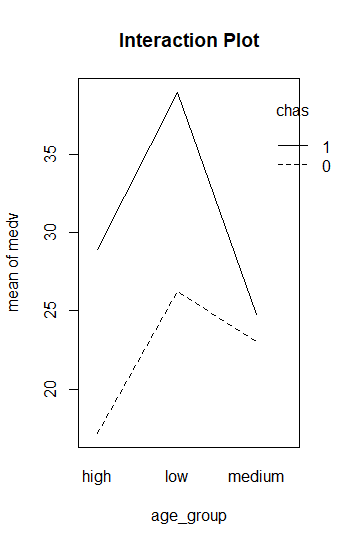
\includegraphics[width=0.4\textwidth]{fig/ex6-2.png}
\end{figure}
\emph{Explanation: age\_group과 chas에 대한 상호작용의 유무를 평균그림을 통해 확인해보자. interaction.plot() 함수를 사용하면 평균 그림을 그릴 수 있고, 두 개의 요인
변수와 관측값을 나타내는 변수를 차례대로 입력해주면 다음과 같은 결과를 얻을 수 있다. 평균 그림 확인 결과, \textbf{두 요인 age\_group과 chas 사이에는 상호작용이 존재하는 것으로 보인다.} } \\

\textbf{(3)} 두 변수 각각의 효과와 두 변수의 교호작용의 유무에 대해 적절한 가설을 쓰고 유의수준 5\%에서 이를 검정하시오.
\begin{lstlisting}[style={r-style}]
fit = lm(medv ~ age_group*chas, data=Boston)
anova(fit)
\end{lstlisting}
\begin{lstlisting}[style={out-style}]

-------------------------------------------------------------------    
Analysis of Variance Table

Response: medv
                Df Sum Sq Mean Sq F value    Pr(>F)    
age_group        2   5852 2925.98 42.6825 < 2.2e-16 ***
chas             1   1736 1735.69 25.3193 6.788e-07 ***
age_group:chas   2    852  426.25  6.2179  0.002151 ** 
Residuals      500  34276   68.55 
---
Signif. codes:  0 '***' 0.001 '**' 0.01 '*' 0.05 '.' 0.1 ' ' 1
-------------------------------------------------------------------
\end{lstlisting}
\emph{Explanation: (반복이 있는 이원배치법의 모형) 
1940년 이전에 지어진 주택의 비율에 따라 만든 속성 age\_group의 주택 가격에 미치는 효과를 $\alpha_i$, Chales River에 대한 더미 변수 chas에 따른 효과를 $\beta_i$, age\_group와 chas의 상호작용을 $\gamma_{ij}$ 라고 하면 검정하고자 하는 가설은 다음과 같다.
(요인 A에 대한) 귀무가설 $H_0: \forall i \  \alpha_i=0$과 대립가설 $H_1$: 적어도 한 $\alpha_i$는 0이 아니다. (요인 B에 대한) 귀무가설 $H_0: \forall i \  \beta_i=0$과 대립가설 $H_1$: 적어도 한 $\beta_i$는 0이 아니다. (교호작용에 대한) 귀무가설 $H_0: \forall i \  \forall j \quad \gamma_{ij}=0$과 대립가설 $H_1$: 적어도 한 $\gamma_{ij}$는 0이 아니다. 상호작용을 포함하는 이원배치 분산분석은 두 개의 요인을 곱(*)으로 표현하여 실행할 수 있다. 분산분석 결과, 유의수준 5\%에서 \textbf{1940년 이전에 지어진 주택의 비율 (A)와 Chales River와 접하는 지 여부 (B)에 따른 상호작용은 존재하는 것}으로 나타났다 (F=6.2179, p-value$<$0.05). 
또한 \textbf{1940년 이전에 지어진 주택의 비율 (A)와 Chales River와 접하는 지 (B) 각각의 요인에 따라서 미치는 주택 가격의 차이가 유의하다}고도 결론 지을 수 있다. (p-value$<$0.05).} \\

\end{document}
